
% --- Page 123 ---
\documentclass{article}
\usepackage{amsmath}
\usepackage{amssymb}
\begin{document}

\section*{3.4 Auflösung von Gleichungen.Implizit definierte Abbildungen 113}

\textbf{Satz über implizite Funktionen}: Sei $I : U \to \mathbb{Z}$ eine $C^1$-Abbildung in einer Umgebung $U \subset X \times Y$ einer Nullstelle $(a, b)$ von $I$. In $(a, b)$ sei das partielle Differential $\partial_y I(a, b)$ invertierbar. Dann gibt es Umgebungen $U' \subset X$ von $a$ und $U'' \subset Y$ von $b$ sowie eine $C^1$-Abbildung $g : U' \to U''$ mit der Eigenschaft, da{\ss} die Nullstellenmenge von $I$ innerhalb $U' \times U''$ genau der Graph von $g$ ist:
$$
I(x,y) = 0, \quad (x,y) \in U' \times U'' \iff y = g(x) , \quad x \in U'.
$$
Man sagt, die Abbildung $g$ sei durch die Gleichung $I(x ,y) = 0$ in der Nähe der Nullstelle $(a, b)$ implizit definiert .

\begin{center}
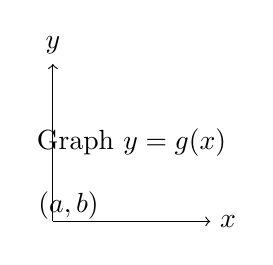
\begin{tikzpicture}
    % Einfache Achsenzeichnung als Platzhalter für das Diagramm
    \draw[->] (0,0) -- (2,0) node[right] {$x$}; 
    \draw[->] (0,0) -- (0,2) node[above] {$y$}; 
    \node at (1,1) {Graph $y=g(x)$}; 
    \node at (0.2, 0.2) {$(a,b)$}; 
\end{tikzpicture}
\end{center}

Die Nullstellenmenge von $f$ innerhalb $U' \times U''$ ist genau der Graph von $g$.

\textbf{Bemerkungen}: 1. Im Fall $X = \mathbb{R}^k$ und $Y = \mathbb{Z} = \mathbb{R}^m$ ist $\partial_y I(a, b)$ genau dann invertierbar , wenn die Matrix $J_I(a,b)$ invertierbar ist.
2. Gelegentlich wird der Satz verkürzt so formuliert : Die L"osungsmannigfaltigkeit der Gleichung $I(x ,y) = 0$ kann in der N"ahe einer L"osung durch $k$ Parameter beschrieben werden; oder auch: Sie besitzt $k$ Freiheitsgrade.
3. Der Satz ist wie der von der lokalen Umkehrbarkeit ein $``$lokaler$''$ Satz : Er stellt nur in hinreichender N"ahe einer gegebenen L"osung die Existenz einer Auflösung fest. Zudem liefert er ein weiteres Beispiel daf{"u}r, da{\ss} sich differenzierbare Abbildungen unter geeigneten Regularit"atsvoraussetzungen lokal wie ihre Linearisierungen verhalten .

\textbf{Beweis}: Wir betrachten die durch $P(x, y) := (x, I(x, y))$ definierte Abbildung $P: U \to X \times Z$. Ihr Differential im Punkt $(a,b)$ ist gegeben durch
$$dP(a,b)(h, k) = (h, \partial_x I(a ,b)h + \partial_y I(a ,b)k), \quad (h, k) \in X \times Y.
$$
Da $\partial_y I(a, b)$ ein Isomorphismus ist, ist auch $dP(a, b)$ ein Isomorphismus. Auf $P$ kann also in $(a, b)$ der Umkehrsatz angewendet werden. Danach gibt es Umgebungen $U_0$ von $(a, b)$ und $V$ von $P(a,b) = (a,0)$ so, da{\ss} die auf $U_0$ eingeschr"ankte Abbildung $P: U_0 \to V$ ein Diffeomorphismus ist.

\end{document}